% !TEX program = pdflatex
\documentclass[aspectratio=169]{beamer}
\usepackage[utf8]{inputenc}
\usepackage[T1]{fontenc}
\usepackage{charter}
% charter.sty sets \bfdefault to b, which beamer's sans body font
% (cmss) lacks, so \textbf
% silently fell back to medium weight; bx exists in both
\renewcommand{\bfdefault}{bx}
\usepackage{amsmath,amssymb}
\usepackage{graphicx}
\usepackage{booktabs}
\usepackage{array}
% Ragged-right paragraph column for tables (no justification or
% hyphenation gaps)
\newcolumntype{L}[1]{>{\raggedright\arraybackslash\hyphenpenalty=10000}p{#1}}
\usepackage{tikz}
\usetikzlibrary{arrows.meta,positioning,calc,fit,decorations.pathreplacing}
\usepackage[most]{tcolorbox}
\tcbuselibrary{raster}
\usepackage{fontawesome5}
\usepackage{dirtree}
\usepackage[backend=bibtex,style=authoryear,maxcitenames=2,natbib=true]{biblatex}
\addbibresource{references.bib}

\graphicspath{{figures/}}

% Oxford Maths (bill) theme; [wellcome] puts the Wellcome logo on the
% title slide
\usetheme{bill}

% Speaker notes
\setbeameroption{hide notes} % Only slides
% \setbeameroption{show only notes} % Only notes
% \setbeameroption{show notes on second screen=right} % Both
\setbeamerfont{note page}{size=\footnotesize}

% Section dividers: contents page with the current section highlighted
% (\tocpage is provided by the bill theme), for every section
% including the first.
% Sections are numbered by the theme, so \section titles below must NOT carry a
% manual "N." prefix. Dividers are numbered like any frame:
% [noframenumbering] would leave
% the footer showing the previous slide's number.
\AtBeginSection[]{
  \begin{frame}
    \tocpage
  \end{frame}
}

% ------------------------------------------------------------------------------------------
% Palette (oxfordblue 0,33,71 comes from the theme)
% ------------------------------------------------------------------------------------------
\definecolor{oxtint}{RGB}{232,238,245}   % soft panel background
\definecolor{oxteal}{RGB}{0,121,140}     % accent: preferred tools,
% key words, links
\definecolor{oxamber}{RGB}{230,126,34}   % importance meter, "you" in diagrams
\definecolor{oxambertext}{RGB}{160,76,0} % darker amber for text on white
\definecolor{oxred}{RGB}{170,26,45}      % risks
\definecolor{oxgrey}{RGB}{96,108,122}    % secondary text, labels
\definecolor{curvegreen}{RGB}{32,142,76} % mitigations; repo-tree
% "good practice"
\definecolor{curveorange}{RGB}{230,126,34}
\definecolor{curvepurple}{RGB}{127,85,170}
\definecolor{termbg}{RGB}{24,30,41}      % demo "terminal" panels
\setbeamercolor{block body}{bg=oxtint}
\newcommand{\key}[1]{\textcolor{oxteal}{\textbf{#1}}}

% Beamer loads hyperref before the preamble, so \PassOptionsToPackage
% has no effect on it;
% set the link colours here. "." keeps theme colours for internal
% links (e.g. the dividers).
\hypersetup{colorlinks=true, urlcolor=oxteal, linkcolor=., citecolor=.}

\DeclareCiteCommand{\citewithjournalurl}
{}
{%
  \printnames{labelname} (\printfield{year}),
  \mkbibemph{\printfield{journaltitle}}%
  \iffieldundef{doi}
  {}
  {, \href{https://doi.org/\thefield{doi}}{https://doi.org/\thefield{doi}}}%
}
{\multicitedelim}
{}

% Pin a paper reference to the bottom-left of the slide, on its own line,
% above the footer. Uses an absolute TikZ overlay so it is independent of the
% frame's vertical alignment and does not disturb the body layout.
\newcommand{\sourceref}[1]{%
  \begin{tikzpicture}[remember picture,overlay]
    \node[anchor=south west, align=left, inner sep=0pt,
      text width=\dimexpr\fullpagewidth-2\titlehmargin\relax,
    xshift=\textmargin, yshift=8.5mm]
    at (current page.south west)
    {\footnotesize\citewithjournalurl{#1}};
  \end{tikzpicture}%
}

% Claude Code docs: \doclink{page}{text} links
% code.claude.com/docs/en/<page> inline;
% \docref{page} pins "Docs: ..." to the bottom-left, in the same
% place as \sourceref.
\newcommand{\doclink}[2]{\href{https://code.claude.com/docs/en/#1}{#2}}
\newcommand{\docref}[1]{%
  \begin{tikzpicture}[remember picture,overlay]
    \node[anchor=south west, align=left, inner sep=0pt,
      text width=\dimexpr\fullpagewidth-2\titlehmargin\relax,
    xshift=\textmargin, yshift=8.5mm]
    at (current page.south west)
    {\footnotesize\color{oxgrey}Docs:
    \href{https://code.claude.com/docs/en/#1}{code.claude.com/docs/en/#1}};
  \end{tikzpicture}%
}

% ------------------------------------------------------------------------------------------
% Practice slides
% ------------------------------------------------------------------------------------------
% Importance meter: n of 5 rounded segments
\newcommand{\meter}[1]{%
  \tikz[baseline=-0.55ex]{\foreach \i in {1,...,5}{%
      \ifnum\i>#1\relax
      \draw[oxfordblue!35, line width=0.6pt, rounded corners=1pt]
      ({(\i-1)*0.34},-0.12) rectangle ++(0.27,0.24);
      \else
      \fill[oxamber, rounded corners=1pt] ({(\i-1)*0.34},-0.12)
      rectangle ++(0.27,0.24);
\fi}}}

% Practice header: \practicehead{fa icon}{score}{one-line pitch}
\newcommand{\practicehead}[3]{%
  \begin{tcolorbox}[enhanced, colback=oxtint, frame hidden, arc=1.5mm,
      left=2mm, right=3mm, top=1mm, bottom=1mm, before skip=1.5mm,
      after skip=1mm,
    borderline west={1.2mm}{0pt}{oxfordblue}]
    \tikz[baseline=-0.7ex]\node[circle, fill=oxfordblue, text=white,
      minimum size=7.5mm,
    inner sep=0pt, font=\normalsize]{\faIcon{#1}};%
    \hspace{2mm}{\large\color{oxfordblue}#3}\hfill
    {\footnotesize\color{oxgrey}Priority}~\meter{#2}
\end{tcolorbox}}

% Tools as chips: \pick = my choice (filled teal), \opt = other tools
% (outlined).
% (\alt is taken by beamer.)
\tikzset{chip/.style={rounded corners=1mm, inner xsep=1.2mm, inner ysep=0.5mm,
text height=1.6ex, text depth=0.45ex, font=\footnotesize}}
\newcommand{\pick}[1]{\tikz[baseline=(c.base)]\node[chip,
    fill=oxteal, text=white,
font=\footnotesize\bfseries](c){#1};}
\newcommand{\opt}[1]{\tikz[baseline=(c.base)]\node[chip,
    draw=oxfordblue!30, fill=white,
text=oxfordblue](c){#1};}
\newtcolorbox{toolpanel}{colback=white, colframe=oxfordblue!20,
  boxrule=0.6pt, arc=1.5mm,
  left=2mm, right=1.5mm, top=1.2mm, bottom=0.6mm, title={\faIcon{tools}~Tools},
  coltitle=oxfordblue, colbacktitle=white, fonttitle=\small\bfseries,
  titlerule=0.4pt, titlerule style=oxfordblue!20,
before upper={\raggedright\lineskip=1.2mm}, before skip=0pt}
% One tool row: grey label in a fixed-width gutter; chips wrap under the chips
\newcommand{\toolrow}[2]{\par\noindent\hangindent=15mm\hangafter=1
\makebox[15mm][l]{\scriptsize\color{oxgrey}#1}#2\par\vspace{0.6mm}}

% Progress through section 1: a row of practice icons, current one filled.
% The icon order must match the order of the practice slides.
\newcommand{\practicetracker}[1]{%
  \begin{tikzpicture}[remember picture, overlay]
    \foreach \ic [count=\k] in {code-branch,boxes,laptop-code,vial,broom,
    project-diagram,spell-check,sync-alt,archive}{%
      \ifnum\k=#1\relax\def\fc{oxfordblue}\def\tc{white}%
      \else\def\fc{oxtint}\def\tc{oxfordblue!45}\fi
      \node[circle, fill=\fc, text=\tc, minimum size=5.2mm, inner sep=0pt,
      font=\scriptsize] at ($(current page.south
      east)+({-\textmargin-2.6mm-(9-\k)*6.2mm},11.5mm)$)
      {\expandafter\faIcon\expandafter{\ic}};
    }
\end{tikzpicture}}

% ------------------------------------------------------------------------------------------
% Diagrams, cards and panels
% ------------------------------------------------------------------------------------------
\tikzset{arr/.style={-{Stealth[length=2mm]}, thick, oxfordblue!70},
  stepbox/.style={rounded corners=1.5mm, minimum height=11mm, align=center,
font=\small, inner sep=1.2mm}}

% Risk card: the risk as the title (red edge); an example line, then
% the mitigation
\newtcolorbox{riskcard}[1]{enhanced, colback=white, colframe=oxfordblue!15,
  boxrule=0.5pt, arc=1.5mm, borderline west={1mm}{0pt}{oxred},
  left=2.5mm, right=2mm, top=0.5mm, bottom=1.5mm, fontupper=\small,
  before upper={\raggedright}, title={#1}, coltitle=oxred, colbacktitle=white,
fonttitle=\small\bfseries, titlerule=0pt, toptitle=1mm, bottomtitle=0mm}
\newcommand{\eg}[1]{{\footnotesize\color{oxgrey}#1\par}\vspace{0.6mm}}
\newcommand{\fix}{\textcolor{curvegreen}{\faIcon{check}}~}

% Prompt example: \begin{promptbox}{edge colour}{title}
\newtcolorbox{promptbox}[2]{enhanced, colback=white, colframe=oxfordblue!15,
  boxrule=0.5pt, arc=1.5mm, borderline west={1mm}{0pt}{#1},
  left=2.5mm, right=2mm,
  top=0.5mm, bottom=1mm, fontupper=\footnotesize, before upper={\raggedright},
  title={#2}, coltitle=#1, colbacktitle=white, fonttitle=\footnotesize\bfseries,
titlerule=0pt, toptitle=1mm, bottomtitle=0mm}

% Content panel: \begin{infopanel}{edge colour}{title}. Amber = you,
% navy = the agent.
\newtcolorbox{infopanel}[2]{enhanced, colback=white, colframe=oxfordblue!15,
  boxrule=0.5pt, arc=1.5mm, borderline west={1.2mm}{0pt}{#1},
  left=3mm, right=2.5mm,
  top=1mm, bottom=2mm, fontupper=\small, before upper={\raggedright},
  title={#2}, coltitle=#1, colbacktitle=white, fonttitle=\bfseries,
titlerule=0pt, toptitle=1.5mm, bottomtitle=0.5mm}

% A column of one-line tiles: \tilestack{icon colour}{icon/text,
% icon/{text, with commas}}
\newcommand{\tilestack}[2]{%
  \begin{tikzpicture}
    \foreach \ic/\txt [count=\k from 0] in {#2}{%
      \node[fill=oxtint, rounded corners=1.5mm, minimum
        width=\linewidth, minimum height=8mm,
      anchor=north west, inner sep=0pt] (t) at (0,-\k*9.8mm) {};
      \node[circle, fill=#1, text=white, minimum size=6mm, inner
      sep=0pt, font=\scriptsize]
      at ([xshift=5mm]t.west) {\expandafter\faIcon\expandafter{\ic}};
      \node[anchor=west, font=\small, inner sep=0pt] at
      ([xshift=10mm]t.west) {\txt};
    }
\end{tikzpicture}}
% Column heading for a stack of tiles: \tileshead{colour}{title}{caption}
\newcommand{\tileshead}[3]{{\large\bfseries\color{#1}#2}\par
\vspace{0.3mm}{\footnotesize\color{oxgrey}#3\par}\vspace{2mm}}

% Instruction-file scope card
\newtcolorbox{scopecard}{enhanced, colback=oxtint, frame hidden,
  arc=1.5mm, left=2mm, right=2mm,
top=1.5mm, bottom=1.5mm, fontupper=\footnotesize, before upper={\raggedright}}

% Demo slides: a dark "terminal" panel with window dots
\newtcolorbox{demobox}{enhanced, colback=termbg, frame hidden, arc=2mm,
  left=5mm, right=5mm, top=7mm, bottom=4mm,
  before upper={\large\setbeamercolor{normal
  text}{fg=white}\usebeamercolor[fg]{normal text}},
  overlay={\foreach \col [count=\n] in {oxred,oxamber,curvegreen}
{\fill[\col] ([xshift=\n*4mm, yshift=-3mm]frame.north west) circle (1.1mm);}}}
\newcommand{\demoitem}{
\item[\textcolor{oxamber}{\faIcon{chevron-right}}]}

% Repo-tree tiers
\newcommand{\ess}[1]{\textcolor{oxambertext}{\textbf{#1}}}
\newcommand{\good}[1]{\textcolor{curvegreen}{#1}}
\newcommand{\choice}{\textsuperscript{*}}
\newcommand{\cmt}[1]{\quad{\sffamily\color{oxgrey}#1}}
\newcommand{\tierkey}[1]{\textcolor{#1}{\rule{0.7em}{0.7em}}}
% dirtree applies \DTstyle inside each entry, so the line spacing
% must be set here too
\renewcommand*\DTstyle{\fontsize{10}{11}\selectfont\ttfamily}
\DTbaselineskip=11pt

\title[Software engineering and AI]{Software engineering
practices\\and AI tools for research code}
\author{William S Hart}
\institute{Infectious Disease Modelling Group\\Mathematical
Institute, University of Oxford}
\date[29 October 2026]{Group meeting, 29 October 2026}

\begin{document}

\begin{frame}[plain]
  \titlepage
\end{frame}

\begin{frame}{This talk}
  \begin{minipage}{\linewidth}
    \large\color{oxfordblue}Check a result, rebuild it reliably, and
    delegate coding
    while retaining scientific control.
  \end{minipage}\par
  \vspace{5mm}
  \begin{itemize}
    \item \textbf{Part 1:} practices and tools for reliable, reproducible code.
    \item \textbf{Part 2:} AI coding tools: uses, good habits and risks.
  \end{itemize}

  \vspace{5mm}
  \begin{tcolorbox}[enhanced, colback=oxamber!10, frame hidden, arc=1.5mm,
      borderline west={1mm}{0pt}{oxamber}, left=3mm, right=3mm,
      top=2mm, bottom=2mm,
    before upper={\raggedright}]
    \small\textbf{Disclaimer:} these slides were prepared with AI
    assistance and may contain
    errors. Check advice against the documentation and your project's needs.
  \end{tcolorbox}
  \note[item]{Allow time for the live repo walkthrough and 8--10
    minutes of discussion.
  Tool panels list options for reference; do not explain every tool.}
\end{frame}

% ==========================================================================================
\section{Practices and tooling}
% ==========================================================================================

\begin{frame}{Organising code}
  \vspace{1mm}
  \centering
  \begin{tikzpicture}[file/.style={stepbox, draw=oxgrey, dashed,
        font=\footnotesize\ttfamily,
      minimum height=8mm},
    scr/.style={stepbox, fill=oxtint, font=\footnotesize}]
    \node[scr] (an)
    {\texttt{final\_size.py}\\{\scriptsize\color{oxgrey}compute, save}};
    \node[file, right=7mm of an] (res) {results/};
    \node[scr, right=7mm of res] (pl)
    {\texttt{final\_size\_plots.py}\\{\scriptsize\color{oxgrey}load, plot}};
    \node[file, right=7mm of pl] (fig) {figures/};
    \draw[arr] (an) -- (res); \draw[arr] (res) -- (pl); \draw[arr]
    (pl) -- (fig);
    \node[stepbox, fill=oxfordblue, text=white, minimum height=9mm,
      anchor=south,
    minimum width=60mm] (pkg) at ($(an.north)!0.5!(pl.north)+(0,9mm)$)
    {\texttt{src/mypkg/}\quad models, likelihoods, helpers};
    \draw[arr] (pkg.south -| an.north) -- node[right,
    font=\scriptsize, text=oxgrey]{import} (an.north);
    \draw[arr] (pkg.south -| pl.north) -- node[right,
    font=\scriptsize, text=oxgrey]{import} (pl.north);
  \end{tikzpicture}\par
  \vspace{2mm}
  \raggedright
  {\small\color{oxgrey}Example: vary $R_0$, compute final sizes, then
  plot the curve.\par}
  \vspace{1mm}
  \begin{itemize}
    \item \textbf{Don't repeat yourself:} put repeated logic in
      functions; define parameters
      once.
    \item \textbf{One function per task:}
      \texttt{compute\_final\_size}, \texttt{plot\_final\_size}.
      Pass inputs explicitly.
    \item \textbf{Public vs private:} keep a small, stable API. In Python, use
      \texttt{\_helper} for private helpers.
  \end{itemize}
  \note[item]{Separating analysis from plotting means figures can be
    tweaked without
  recomputing.}
  \note[item]{Replace copy-pasted logic with a function so fixes
    apply everywhere. Define
    parameters such as the recovery rate once; repeating a one-liner
    can be fine. Avoid hidden
    globals. Private helpers can change without changing the public
    API; Python's leading
  underscore is a convention, not access control.}
\end{frame}

\begin{frame}{Nine practices: my adoption priorities}
  \centering
  \begin{tikzpicture}[tile/.style={rounded corners=1.5mm,
        fill=oxtint, minimum width=46mm,
    minimum height=13mm}]
    \foreach \ic/\name/\sc [count=\k from 0] in {code-branch/Version control/5,
      boxes/Environments/5, laptop-code/Editor and debugger/5,
      vial/Formal testing/4,
      broom/Formatting and linting/3, project-diagram/Workflow management/3,
      spell-check/Type checking/2, sync-alt/Continuous integration/2,
    archive/Archiving code/2}{%
      \pgfmathsetmacro{\cx}{mod(\k,3)*49}\pgfmathsetmacro{\cy}{-int(\k/3)*16}
      \node[tile, anchor=north west] (t) at (\cx mm,\cy mm) {};
      \node[circle, fill=oxfordblue, text=white, minimum size=7mm,
      inner sep=0pt]
      at ([xshift=6mm]t.west) {\expandafter\faIcon\expandafter{\ic}};
      \node[anchor=north west, font=\footnotesize\bfseries,
      text=oxfordblue, inner sep=0pt]
      at ([xshift=11mm, yshift=-2.2mm]t.north west) {\name};
      \node[anchor=south west, inner sep=0pt] at ([xshift=11mm,
      yshift=2.2mm]t.south west)
      {\meter{\sc}};
    }
  \end{tikzpicture}\par
  \vspace{4mm}
  \begin{tcolorbox}[enhanced, colback=oxtint, frame hidden,
      arc=1.5mm, left=3mm, right=3mm,
    before skip=0pt, after skip=0pt, before upper={\raggedright}]
    \small
    \meter{5}~~Priority for a typical analysis repo (5 = start here)\par
    \vspace{1.5mm}
    \pick{my choice}~\opt{other tools}~~Tools for Python, R and Julia
  \end{tcolorbox}
  \note[item]{These are personal adoption priorities, not a universal
    ranking. Basic
    scientific checks are essential; the testing score refers to a
    formal test suite.
  Organisation and documentation underpin all nine practices.}
\end{frame}

\begin{frame}[t]{Version control}
  \practicehead{code-branch}{5}{Record changes; restore committed versions.}
  \begin{columns}[t]
    \column{0.54\textwidth}\vspace{0pt}
    \begin{itemize}
      \item See what changed, when and why.
      \item Push to a remote for backup and collaboration.
      \item Branches let features develop in parallel.
      \item Commit before an agent edits, then review its diff.
    \end{itemize}

    \column{0.42\textwidth}\vspace{0pt}
    \begin{toolpanel}
      \toolrow{Any}{\pick{git}}
      \toolrow{Hosting}{\pick{GitHub} \opt{GitLab}}
      \toolrow{Interfaces}{\opt{VS Code} \opt{GitHub Desktop}
      \opt{GitHub CLI (gh)}}
    \end{toolpanel}
  \end{columns}
  \practicetracker{1}
  \note[item]{Commit small and often, with messages that say why.}
  \note[item]{Git records committed files, not arbitrary command
    effects or untracked data.
    See
  \url{https://git-scm.com/book/en/v2/Git-Basics-Recording-Changes-to-the-Repository}.}
  \note[item]{Git worktrees are extra checkouts of the repo on other
    branches, so several
  agent sessions can work at once (part 2).}
\end{frame}

\begin{frame}[t]{Environments and package management}
  \practicehead{boxes}{5}{A recorded environment for each project.}
  \begin{columns}[t]
    \column{0.54\textwidth}\vspace{0pt}
    \begin{itemize}
      \item Code depends on package versions (e.g.\ numpy~2).
      \item A shared global environment drifts and breaks old projects.
      \item Commit an environment specification with package versions.
      \item A lockfile also records resolved dependencies, making
        rebuilding easier.
    \end{itemize}

    \column{0.42\textwidth}\vspace{0pt}
    \begin{toolpanel}
      \toolrow{Python}{\pick{pixi} \opt{uv} \opt{conda/mamba} \opt{pip + venv}}
      \toolrow{R}{\pick{renv} \opt{pak} \opt{rig}}
      \toolrow{Julia}{\opt{Pkg}}
      \toolrow{Containers}{\opt{Docker} \opt{Apptainer}}
    \end{toolpanel}
  \end{columns}
  \practicetracker{2}
  \note[item]{pixi installs from conda-forge and PyPI, with a
    cross-platform lockfile and
    tasks; it handles R and non-Python dependencies too. uv is
    excellent if everything is on
    PyPI. pak installs R packages and can complement renv; rig
    manages R versions and now
  has experimental project management.}
  \note[item]{The score is for recording the environment, not
    requiring a lockfile. A pinned
    requirements.txt can be sufficient. Record Python/R versions and
    any system requirements
    too; a lockfile only covers its supported platforms and managed
    dependencies.
  See \url{https://pixi.prefix.dev/latest/workspace/system_requirements/}.}
\end{frame}

\begin{frame}[t]{Editor and debugger}
  \practicehead{laptop-code}{5}{Navigate code and catch errors as you type.}
  \begin{columns}[t]
    \column{0.54\textwidth}\vspace{0pt}
    \begin{itemize}
      \item The editor flags errors and makes code easy to navigate.
      \item A debugger pauses the code so you can inspect its state.
      \item Work with AI agents, then review and edit their changes
        in the editor.
    \end{itemize}

    \column{0.42\textwidth}\vspace{0pt}
    \begin{toolpanel}
      \toolrow{Editors}{\pick{VS Code} \opt{PyCharm} \opt{Positron}
      \opt{RStudio}}
      \toolrow{Debuggers}{\pick{VS Code debugger} \opt{pdb} \opt{R browser()}
      \opt{Infiltrator.jl}}
    \end{toolpanel}
  \end{columns}
  \practicetracker{3}
  \note[item]{The score is for using a capable editor. Learning to
    use its debugger is a
  useful next step.}
  \note[item]{Agents can run inside the editor or in a separate
    terminal. Either way, open
    their changes in the editor to inspect the diff, make corrections
  and run or debug code.}
  \note[item]{For notebooks, restart the kernel and run all cells in
    order. Put reusable
    logic in the package. The script-pair layout is my preference, not
  a requirement.}
\end{frame}

\begin{frame}[t]{Formal testing}
  \practicehead{vial}{4}{Automate checks as your code changes.}
  \begin{columns}[t]
    \column{0.54\textwidth}\vspace{0pt}
    \begin{itemize}
      \item \textbf{Basic checks are essential.} The score is for a
        formal test suite.
      \item Start with simple cases where you know the right answer.
      \item Cover edge cases and important rules, e.g.\ totals
        adding up.
      \item When you fix a bug, add a test to catch it if it returns.
    \end{itemize}

    \column{0.42\textwidth}\vspace{0pt}
    \begin{toolpanel}
      \toolrow{Python}{\pick{pytest} \opt{hypothesis} \opt{pytest-cov}}
      \toolrow{R}{\pick{testthat}}
      \toolrow{Julia}{\opt{Test}}
    \end{toolpanel}
  \end{columns}
  \practicetracker{4}
  \note[item]{Run the tests after changes to check that working code still behaves as
    expected. Edge cases include empty inputs, zero rates or boundary values, depending on
    the function. Test-driven development is one option: write a failing test, then implement
    the behaviour it specifies.}
  \note[item]{Tests build confidence that the implementation matches
    the model, and provide
    regression checks when refactoring. Examples: population
    conservation, non-negativity,
  and convergence as solver tolerances tighten.}
  \note[item]{Simulate-and-recover: check recovery and uncertainty
    across simulated datasets.
    A single noisy or weakly identified dataset need not recover the
    generating parameters.
    See
  \url{https://mc-stan.org/docs/stan-users-guide/simulation-based-calibration.html}.}
  \note[item]{Stochastic code: pass \texttt{rng =
    np.random.default\_rng(seed)} into functions
    rather than setting a global seed; test with
    \texttt{assert\_allclose} or statistical
    tolerances where appropriate. A seed alone does not guarantee the
    same results across
    builds and platforms:
  \url{https://numpy.org/doc/stable/reference/random/compatibility.html}.}
  \note[item]{With an agent: write or approve the test yourself, then
    ask it to make the test
    pass without editing it. hypothesis does property-based testing;
    pytest-cov measures
  coverage.}
\end{frame}

\begin{frame}[t]{Formatting and linting}
  \practicehead{broom}{3}{Consistent style; common mistakes flagged.}
  \begin{columns}[t]
    \column{0.54\textwidth}\vspace{0pt}
    \begin{itemize}
      \item \textbf{Formatters} standardise spacing and line breaks.
      \item \textbf{Linters} flag likely bugs and bad patterns
        without running the code,
        e.g.\ undefined names, unused imports.
      \item Both run on save, or after each agent edit (a hook: a command run
        automatically).
    \end{itemize}

    \column{0.42\textwidth}\vspace{0pt}
    \begin{toolpanel}
      \toolrow{Python}{\pick{ruff} \opt{pylint}}
      \toolrow{R}{\opt{air} \opt{styler} \opt{lintr}}
      \toolrow{Julia}{\opt{JuliaFormatter.jl} \opt{Runic.jl}}
      \toolrow{Any}{\opt{pre-commit}}
    \end{toolpanel}
  \end{columns}
  \practicetracker{5}
  \note[item]{ruff replaces black, isort and flake8 in one fast tool.
    pre-commit runs checks
  before each commit.}
\end{frame}

\begin{frame}[t]{Workflow management}
  \practicehead{project-diagram}{3}{One command rebuilds every result.}
  \begin{columns}[t]
    \column{0.54\textwidth}\vspace{0pt}
    \begin{itemize}
      \item Reruns affected steps when declared inputs change.
      \item Makes the dependencies between data, code and outputs explicit.
      \item Can run jobs on HPC clusters as projects grow.
    \end{itemize}

    \column{0.42\textwidth}\vspace{0pt}
    \begin{toolpanel}
      \toolrow{Any}{\pick{Snakemake} \opt{Nextflow} \opt{Make}}
      \toolrow{R}{\opt{targets}}
      \toolrow{Simple}{\opt{pixi tasks}}
    \end{toolpanel}
  \end{columns}
  \practicetracker{6}
  \note[item]{Snakemake works with any language, Julia included: each
    rule just runs a
  command.}
  \note[item]{Running example: changing the R0 grid should recompute
    final sizes and then
    redraw the curve; changing only the plot style should redraw it
    without recomputing.
  Record parameter values and units with results.}
\end{frame}

\begin{frame}[t]{Type checking}
  \practicehead{spell-check}{2}{Catch wrong-type bugs before running.}
  \begin{columns}[t]
    \column{0.54\textwidth}\vspace{0pt}
    \begin{itemize}
      \item E.g.\ passing \texttt{None} where an array is expected.
      \item Type hints document interfaces, and help editors and AI.
      \item Useful for stable interfaces; AI can help add hints.
    \end{itemize}

    \column{0.42\textwidth}\vspace{0pt}
    \begin{toolpanel}
      \toolrow{Python}{\pick{ty (beta)} \opt{pyrefly} \opt{mypy} \opt{pyright}}
      \toolrow{Julia}{\opt{JET.jl}}
      \toolrow{R}{{\scriptsize\color{oxgrey}none mainstream}}
    \end{toolpanel}
  \end{columns}
  \practicetracker{7}
  \note[item]{} % Add notes here
\end{frame}

\begin{frame}[t]{Continuous integration}
  \practicehead{sync-alt}{2}{Tests run on every push, on clean machines.}
  \begin{columns}[t]
    \column{0.54\textwidth}\vspace{0pt}
    \begin{itemize}
      \item Catches ``works on my machine'' and broken lockfiles.
      \item Can test several operating systems.
      \item Analysis repos can run a small smoke test; shared
        packages need fuller checks.
    \end{itemize}
    \vspace{1mm}
    {\footnotesize\color{oxgrey}Packages other people install:}~\meter{4}

    \column{0.42\textwidth}\vspace{0pt}
    \begin{toolpanel}
      \toolrow{Pipelines}{\pick{GitHub Actions} \opt{GitLab CI}}
      \toolrow{Coverage}{\pick{Codecov}}
    \end{toolpanel}
  \end{columns}
  \practicetracker{8}
  \note[item]{} % Add notes here
\end{frame}

\begin{frame}[t]{Archiving code}
  \practicehead{archive}{2}{A permanent copy of the code behind each paper.}
  \begin{columns}[t]
    \column{0.54\textwidth}\vspace{0pt}
    \begin{itemize}
      \item A one-off step at publication: archive the exact version
        used for the paper.
      \item A DOI keeps the paper's link permanent, even if the repo moves.
      \item Zenodo's GitHub integration needs a public repo;
        otherwise upload the release by
        hand.
    \end{itemize}
    \vspace{1mm}
    {\footnotesize\color{oxgrey}At publication:}~\meter{4}

    \column{0.42\textwidth}\vspace{0pt}
    \begin{toolpanel}
      \toolrow{Archives}{\pick{Zenodo} \opt{Software Heritage} \opt{OSF}}
    \end{toolpanel}
  \end{columns}
  \practicetracker{9}
  \note[item]{Zenodo archives each GitHub release automatically once
    the repo is public, and
  gives a citation if one is needed.}
\end{frame}

\begin{frame}{What goes in a repo}
  \begin{columns}[T]
    \column{0.7\textwidth}
    \dirtree{%
      .1 project/.
      .2 \ess{README.md}\cmt{what it is, install, reproduce}.
      .2 \ess{LICENSE}\cmt{no licence = no reuse}.
      .2 \ess{.gitignore}.
      .2 \ess{pyproject.toml\choice}\cmt{environment spec}.
      .2 \good{pixi.lock\choice}\cmt{exact versions}.
      .2 \good{AGENTS.md\choice}\cmt{project instructions}.
      .2 \good{src/mypkg/\choice}\cmt{reusable code as a package}.
      .2 \good{scripts/\choice}\cmt{analysis + plot script pairs}.
      .3 \good{final\_size.py}\cmt{compute, save results}.
      .3 \good{final\_size\_plots.py}\cmt{load results, plot}.
      .2 \good{tests/}.
      .2 \good{data/}\cmt{inputs and provenance; no sensitive data}.
      .2 \good{results/}\cmt{outputs (committed: my choice)}.
      .2 \good{figures/}.
      .2 \good{Snakefile\choice}\cmt{reproduction workflow}.
    }

    \column{0.27\textwidth}
    {\small
      \tierkey{oxambertext}~\textbf{Essential}\par\vspace{2mm}
    \tierkey{curvegreen}~Good practice\par}
    \vspace{5mm}
    {\small\color{oxgrey}Colour rates the practice.\par
      \vspace{3mm}\choice~My choice of format, tool or layout;
    alternatives work too.}
  \end{columns}
  \note[item]{Show the live repo here. Alternatives: uv or conda
    environment.yml; a flat
    package instead of src layout; notebooks instead of script pairs;
    regenerating outputs
    instead of committing them; pixi tasks or Make instead of
    Snakemake. The environment
  specification is essential; pyproject.toml is my choice of format.}
  \note[item]{This repo has CLAUDE.md importing AGENTS.md. Keep
    identifiable data and secrets
  outside the repo; record data sources, versions and access instructions.}
\end{frame}

\begin{frame}{Documenting code}
  \begin{itemize}
    \item README: what it is, how to install it, how to reproduce the results.
    \item Docstrings (roxygen comments in R): purpose, arguments,
      units, returns.
    \item Comments say \emph{why}, not \emph{what}.
    \item Names say what things are (\texttt{incubation\_period}, not
      \texttt{ip}).
    \item Delete commented-out code. Retrieve committed versions from git.
    \item Doc websites are useful for shared packages: \pick{Sphinx}
      \opt{roxygen2 + pkgdown}
      \opt{Documenter.jl}
  \end{itemize}
  \note[item]{Python docstrings in Google or NumPy style.}
\end{frame}

\begin{frame}{Additional resources}
  \begin{itemize}
    \item \emph{Best practices for scientific computing}:\\
      \citewithjournalurl{wilson2014best}
    \item \emph{Good enough practices in scientific computing}:\\
      \citewithjournalurl{wilson2017good}
    \item \emph{The Turing Way}, a handbook for reproducible research:\\
      \url{https://book.the-turing-way.org}
    \item Oxford Research Software Engineering group training:\\
      \url{https://www.rse.ox.ac.uk/training}
  \end{itemize}
  \note[item]{} % Add notes here
\end{frame}

% ==========================================================================================
\section{AI tools}
% ==========================================================================================

\begin{frame}{Options: chat assistants and coding agents}
  \begin{tikzpicture}[b/.style={stepbox, fill=oxtint, text
      width=19mm, minimum height=10mm},
      you/.style={circle, fill=oxamber!25, draw=oxamber, minimum size=10mm},
      lb/.style={font=\scriptsize, text=oxgrey},
      t/.style={stepbox, fill=oxtint, minimum height=6mm,
        font=\scriptsize, inner sep=0.8mm,
    text width=11mm}]
    % chat row
    \node[anchor=west, text width=27mm, align=left] (h1) at (0,0)
    {\textbf{Chat}\\{\footnotesize\color{oxgrey}ChatGPT, claude.ai}};
    \node[b, right=2mm of h1] (chat) {\faIcon{comments}\\Chat};
    \node[you, right=12mm of chat] (you) {\faIcon{user}};
    \node[b, right=12mm of you] (ed) {\faIcon{laptop-code}\\Editor};
    \draw[arr] ([yshift=1.5mm]chat.east) -- node[lb, above]{copy
    code} ([yshift=1.5mm]you.west);
    \draw[arr] ([yshift=-1.5mm]you.west) -- node[lb, below]{paste
    errors} ([yshift=-1.5mm]chat.east);
    \draw[arr] ([yshift=1.5mm]you.east) -- node[lb, above]{run}
    ([yshift=1.5mm]ed.west);
    \draw[arr] ([yshift=-1.5mm]ed.west) -- node[lb, below]{errors}
    ([yshift=-1.5mm]you.east);
    \node[anchor=west, text width=33mm, font=\small] at ([xshift=3mm]ed.east)
    {\textcolor{oxambertext}{\textbf{You}} are the loop. Good for
    questions, snippets.};
    % agent row
    \node[anchor=west, text width=27mm, align=left] (h2) at (0,-24mm)
    {\textbf{Coding agent}\\{\footnotesize\color{oxgrey}Claude Code, Codex}};
    \node[you, right=6.5mm of h2] (you2) {\faIcon{user}};
    \node[circle, fill=oxfordblue, text=white, minimum size=10mm,
    right=17mm of you2] (ag) {\faIcon{robot}};
    \draw[arr] ([yshift=1.5mm]you2.east) -- node[lb, above]{prompt}
    ([yshift=1.5mm]ag.west);
    \draw[arr] ([yshift=-1.5mm]ag.west) -- node[lb, below]{diffs}
    ([yshift=-1.5mm]you2.east);
    \node[t, right=8mm of ag, yshift=3.5mm] (f) {files};
    \node[t, right=2mm of f] (r) {run};
    \node[t, right=8mm of ag, yshift=-3.5mm] (te) {tests};
    \node[t, right=2mm of te] (g) {git};
    \node[draw=oxgrey, dashed, rounded corners=1.5mm,
    fit=(f)(r)(te)(g), inner sep=1.5mm] (repo) {};
    \draw[arr, <->] (ag) -- (repo);
    \node[anchor=west, text width=33mm, font=\small] at
    ([xshift=3mm]ed.east |- ag)
    {\textcolor{oxfordblue}{\textbf{It}} runs the loop in your repo;
    you review.};
  \end{tikzpicture}

  \vspace{5mm}
  {\footnotesize
    \pick{Claude Code} {\color{oxgrey}terminal, VS Code, desktop, web}\quad
    \pick{OpenAI Codex} {\color{oxgrey}CLI, IDE, cloud}\par
    \vspace{1mm}
  {\color{oxgrey}Also: GitHub Copilot (agent mode), Cursor, Gemini CLI.}\par}
  \note[item]{} % Add notes here
\end{frame}

\begin{frame}{How much to delegate}
  \centering
  \begin{tikzpicture}
    \shade[left color=oxamber, right color=oxfordblue, rounded
    corners=1mm] (0,-0.07) rectangle (14,0.07);
    \node[anchor=north west, font=\footnotesize, text=oxgrey] at (0,-0.15)
    {You do more};
    \node[anchor=north east, font=\footnotesize, text=oxgrey] at (14,-0.15)
    {AI does more};
    \foreach \x/\col/\name/\desc in {%
      2/oxamber/{You write, AI assists}/{Autocomplete, explanations,
        reviewing your code.
      More hands-on practice.},
      7/oxgrey/Smaller chunks/{One function or feature at a time,
      reading every diff.},
      12/oxfordblue/Full vibe/{Accepting code without reading it.
        Throwaway exploration;
      check any result you use.}%
    }{%
      \fill[white] (\x,0) circle (0.2); \fill[\col] (\x,0) circle (0.14);
      \node[anchor=base, font=\bfseries] at (\x,0.45) {\name};
      \node[anchor=north, text width=4.2cm, align=left, font=\small,
      execute at begin node={\hyphenpenalty=10000}] at (\x,-0.8) {\desc};
    }
  \end{tikzpicture}
  \note[item]{Full vibe can be useful for throwaway exploration. A
    plot can influence your
    scientific decisions before publication, so check anything you
    rely on. Use the left or
    middle for research outputs; the total time saved depends on
  verification and rework.}
\end{frame}

\begin{frame}{Plan the science before the code}
  \begin{minipage}{\textwidth}
    \textbf{Make scientific choices explicit, or the agent will
    choose defaults.}
  \end{minipage}
  \vspace{2mm}
  \begin{tcbraster}[raster columns=2, raster equal height=rows,
    raster column skip=4mm]
    \begin{infopanel}{oxambertext}{\faIcon{user}~Specify the analysis}
      \begin{itemize}
        \item Scientific question, model assumptions and data.
        \item Parameters, priors and their sources.
        \item Inference, diagnostics and checks against data or known answers.
      \end{itemize}
      \vspace{1mm}
      {\color{oxgrey}Record the agreed choices in a brief the agent
      can implement.}
    \end{infopanel}
    \begin{infopanel}{oxfordblue}{\faIcon{robot}~AI can help develop it}
      \begin{itemize}
        \item Compare modelling or inference approaches.
        \item Work through derivations, e.g.\ the final-size relation.
        \item Suggest limiting cases and checks.
      \end{itemize}
      \vspace{1mm}
      \fix Verify the maths and approve the specification.
    \end{infopanel}
  \end{tcbraster}
  \note[item]{Anything left unspecified may be decided by the agent:
    a default prior, an
    optimiser, a parameterisation. Code matching the equations is
    separate from the model
    adequately answering the scientific question; include checks
    against data and sensitivity
  to assumptions.}
  \note[item]{E.g.\ ask it to derive the final size relation for your
    model, then check it
  with SymPy or against a simulation.}
  \note[item]{This is the scientific specification; the later
    planning slide covers the
    implementation plan. Exploration can inform the specification,
    and it can evolve: revise
  the scientific choices explicitly as you learn.}
\end{frame}

\begin{frame}{Uses: checking and testing}
  \begin{itemize}
    \item \textbf{Bugs:} share the traceback and a reproducible
      example. Ask it to explain
      the cause and verify the fix.
    \item \textbf{Tests:} AI can help write unit tests, suggest edge
      cases and extend coverage.
  \end{itemize}
  \vspace{3mm}
  {\small\textbf{Example requests}\par}
  \vspace{2mm}
  \begin{tcbraster}[raster columns=2, raster equal height=rows,
    raster column skip=4mm]
    \begin{infopanel}{oxfordblue}{Review code}
      ``Compare this implementation with the model description.
      Report suspected bugs with file and line references, and
      examples that demonstrate each issue. Do not edit yet.''
    \end{infopanel}
    \begin{infopanel}{oxteal}{Extend tests}
      ``Read this module and its existing tests. Identify untested
      behaviours, add unit tests following the existing style,
      and run them. Show the new tests and their results.''
    \end{infopanel}
  \end{tcbraster}
  \note[item]{For a review, supply the relevant code and scientific specification, such as
    equations, a paper's methods or an agreed analysis brief. Ask for concrete findings so
    you can assess them before requesting changes; a second session can review your code or
    another agent's work. Follow confirmed findings with a fix and a regression test.}
  \note[item]{For test writing, point the agent to the module and existing suite. It can
    inspect the public functions, suggest missing cases, write the test code, run it and
    investigate failures. Review its expected answers and the diff, including changes to
    existing tests. Ask for the command and actual output, rather than a claim that tests pass.}
\end{frame}

\begin{frame}[t]{Uses: grunt work and more}
  \vspace{2mm}
  \begin{columns}[t]
    \column{0.47\textwidth}\vspace{0pt}
    \tileshead{oxfordblue}{Grunt work}{Tedious for you, quick for you to check.}
    \tilestack{oxfordblue}{tags/Type hints and docstrings,
      exchange-alt/Renames across files,
      clone/New-but-similar sensitivity analyses,
      compress-arrows-alt/Turning copy-paste into functions,
    arrow-circle-up/Updating for new library versions}

    \column{0.47\textwidth}\vspace{0pt}
    \tileshead{oxteal}{And more}{Reading, translating, explaining.}
    \tilestack{oxteal}{book-open/Understanding unfamiliar code,
      language/Translating R or MATLAB to Python,
      bug/Decoding install and HPC errors,
      file-alt/{READMEs, commits, merge conflicts},
    chalkboard/Slides for a supervisor meeting}
  \end{columns}
  \note[item]{Grunt work is where agents shine: tedious to do, but
    the result is quick to
  check. New sensitivity analyses: point it at an existing one to follow.}
  \note[item]{Understanding unfamiliar code: a paper's repo, or a new library.}
\end{frame}

\begin{frame}{Prompting}
  \begin{itemize}
    \item \textbf{Give context:} the symptom, relevant files and
      constraints. Point to a
      pattern if useful.
    \item \textbf{Define success:} expected behaviour and a check it
      can run. Ask for evidence.
    \item \textbf{Unclear scope:} ask it to interview you and write a
      brief specification.
    \item \textbf{Exploring:} open questions are fine (``what would
      you improve here?'').
  \end{itemize}

  \vspace{2mm}
  \begin{columns}[T]
    \column{0.33\textwidth}
    \begin{promptbox}{oxred}{Vague}
      ``fix the bug in the plot''
    \end{promptbox}
    \column{0.63\textwidth}
    \begin{promptbox}{curvegreen}{Specific}
      ``The final-size plot shows 0.2 on an axis labelled (\%). In
      \texttt{scripts/final\_size\_plots.py}, make 0.2 display as
      20\%, keeping saved results
      as fractions. Regenerate and show the figure.''
    \end{promptbox}
  \end{columns}
  \docref{best-practices}
  \note[item]{The linked best-practices guide recommends supplying
    information the agent
    cannot infer, naming the symptom and expected behaviour,
    providing a check it can run,
    and asking for concrete evidence. If scope is unclear, interview
    first and write a spec.
  Open-ended prompts are appropriate for exploration.}
  \note[item]{The example specifies the observable bug, a file, the
    desired result and a
    constraint on scope. The evidence is the regenerated figure. A
    traceback, screenshot,
  small input or failing test can provide more context when relevant.}
\end{frame}

\begin{frame}{Planning with an agent}
  \centering
  \begin{tikzpicture}[node distance=4mm,
      ro/.style={stepbox, fill=oxtint, text=oxfordblue, text
      width=17mm, minimum height=12.5mm},
      you/.style={stepbox, fill=oxamber!18, draw=oxamber, text
      width=17mm, minimum height=12.5mm},
      rw/.style={stepbox, fill=oxfordblue, text=white, text width=17mm,
    minimum height=12.5mm}]
    \node[you] (in) {\faIcon{comment}\\Describe task};
    \node[ro, right=of in] (ex) {\faIcon{search}\\Explore};
    \node[ro, right=of ex] (pl) {\faIcon{clipboard-list}\\Write plan};
    \node[you, right=of pl] (rv) {\faIcon{user-check}\\Review};
    \node[rw, right=11mm of rv] (im) {\faIcon{code}\\Implement};
    \node[rw, right=of im] (ck) {\faIcon{check-double}\\Test, report};
    \draw[arr] (in) -- (ex); \draw[arr] (ex) -- (pl); \draw[arr] (pl) -- (rv);
    \draw[arr] (rv) -- node[above, font=\scriptsize, text=oxgrey]{approve} (im);
    \draw[arr] (im) -- (ck);
    \draw[arr] (rv.south) to[out=-130, in=-50] node[below,
    font=\scriptsize, text=oxgrey]{revise} (pl.south);
  \end{tikzpicture}\par
  \vspace{0.5mm}
  {\scriptsize\color{oxgrey}
    \tikz\draw[fill=oxamber!18, draw=oxamber] (0,0) rectangle
    (0.25,0.25);~you\qquad
    \tikz\fill[oxtint] (0,0) rectangle (0.25,0.25);~agent, read-only
    (no file changes)\qquad
  \tikz\fill[oxfordblue] (0,0) rectangle (0.25,0.25);~agent, editing\par}

  \vspace{2mm}
  \raggedright
  \begin{tcbraster}[raster columns=2, raster equal height=rows,
    raster column skip=4mm]
    \begin{infopanel}{curvegreen}{\faIcon{check}~Use it}
      When you're unsure of the approach, or several files change:
      use plan mode, or ask
      for a plan and no edits.
    \end{infopanel}
    \begin{infopanel}{oxred}{\faIcon{times}~Skip it}
      For small, well-understood edits.
    \end{infopanel}
  \end{tcbraster}
  \docref{permission-modes}
  \note[item]{In Claude Code: \texttt{Shift+Tab} cycles modes (three
    presses from auto), or
  start a single prompt with \texttt{/plan}.}
  \note[item]{This talk was planned this way.}
  \note[item]{After implementation, review the diff and test evidence
  before committing.}
\end{frame}

\begin{frame}[t]{Sessions and context}
  \vspace{2mm}
  \begin{tikzpicture}[bar/.style={draw=oxfordblue!40, rounded
        corners=1mm, minimum height=6mm,
      minimum width=72mm, anchor=west},
      seg/.style={minimum height=6mm, anchor=west, inner sep=0pt,
      font=\scriptsize},
      lab/.style={anchor=east, font=\footnotesize\ttfamily, text=oxfordblue},
      note/.style={anchor=west, font=\footnotesize, text=oxgrey, text
        width=46mm,
    execute at begin node={\hyphenpenalty=10000}}]
    % row 1: full context
    \node[lab] at (0,0) {full};
    \shade[left color=oxtint, right color=oxred!45, rounded corners=1mm]
    (2mm,-3mm) rectangle ++(72mm,6mm);
    \node[seg, fill=oxfordblue, text=white, minimum width=21mm, inner
    xsep=1mm] at (2mm,0) {AGENTS.md};
    \node[seg, text=oxfordblue] at (25mm,0) {task A \dots};
    \node[seg, text=white] at (50mm,0) {task B \dots};
    \node[note] at (76mm,0) {Long, mixed context can reduce quality.};
    % row 2: /clear
    \node[lab] at (0,-9mm) {fresh};
    \node[bar] at (2mm,-9mm) {};
    \node[seg, fill=oxfordblue, text=white, minimum width=21mm, inner
    xsep=1mm] at (2mm,-9mm) {AGENTS.md};
    \node[note] at (76mm,-9mm) {New session between unrelated tasks.};
    % row 3: compacted
    \node[lab] at (0,-18mm) {compacted};
    \node[bar] at (2mm,-18mm) {};
    \node[seg, fill=oxfordblue, text=white, minimum width=21mm, inner
    xsep=1mm] at (2mm,-18mm) {AGENTS.md};
    \node[seg, fill=oxteal, text=white, minimum width=17mm, inner
    xsep=1mm] at (24mm,-18mm) {summary};
    \node[note] at (76mm,-18mm) {Summarise between linked tasks,
    saying what to keep.};
  \end{tikzpicture}

  \vspace{3mm}
  \begin{itemize}
    \item Two failed corrections? Start afresh with a better prompt.
    \item Interrupt early. Checkpoints restore captured edits; git
      restores committed files.
      Neither reverses every command.
    \item Review in a fresh session or with a second model to reduce anchoring.
  \end{itemize}
  \docref{best-practices}
  \note[item]{Long sessions compact automatically, so details can be
    lost; compact yourself
    between linked tasks, e.g.\ once a long debugging session has found
  the cause.}
  \note[item]{In Claude Code: \texttt{/clear}, \texttt{/compact <what to keep>},
    \texttt{Esc} to stop, \texttt{Esc Esc} or \texttt{/rewind} to undo,
    \texttt{claude -{}-continue}/\texttt{-{}-resume} to pick up
    later, and git worktrees for
  parallel sessions.}
  \note[item]{Fresh review can repeat the same mistaken assumptions.
    Give the reviewer the
    scientific specification and checks; retain human scientific
    review. Checkpoint limits:
  \url{https://code.claude.com/docs/en/checkpointing}.}
\end{frame}

\begin{frame}{Agent instruction files}
  \begin{tcbraster}[raster columns=3, raster equal height=rows,
    raster column skip=2.5mm]
    \begin{scopecard}
      \textcolor{oxfordblue}{\faIcon{users}}~\textbf{Project}\par
      \vspace{1mm}{\color{oxgrey}Committed (\texttt{AGENTS.md}): the
        project's conventions,
      for everyone.}
    \end{scopecard}
    \begin{scopecard}
      \textcolor{oxfordblue}{\faIcon{user-lock}}~\textbf{Personal,
      this project}\par
      \vspace{1mm}{\color{oxgrey}Your preferences; not committed.}
    \end{scopecard}
    \begin{scopecard}
      \textcolor{oxfordblue}{\faIcon{user}}~\textbf{Personal, all projects}\par
      \vspace{1mm}{\color{oxgrey}In your home config.}
    \end{scopecard}
  \end{tcbraster}

  \vspace{2mm}
  \begin{itemize}
    \item Loaded every session: commands and conventions the agent can't infer.
    \item Keep it short: would removing this line cause mistakes?
    \item Add a rule when you find yourself repeating a correction.
    \item \texttt{AGENTS.md} is an open format read by many coding agents.
  \end{itemize}
  \docref{memory}
  \note[item]{In Claude Code: personal files are
    \texttt{CLAUDE.local.md} (add it to
    \texttt{.gitignore}) and
    \texttt{\textasciitilde/.claude/CLAUDE.md}; \texttt{/init} drafts a
    first version. Claude Code reads \texttt{AGENTS.md} directly only
    when there is no
    \texttt{CLAUDE.md} or \texttt{CLAUDE.local.md}, so this repo's
    \texttt{CLAUDE.md} imports it
  with \texttt{@AGENTS.md}.}
\end{frame}

\begin{frame}{Skills}
  \begin{itemize}
    \item Instructions plus templates and scripts, loaded when
      relevant or on request.
    \item Load detailed procedures when needed.
    \item \textbf{Make one} ``when you keep pasting the same
      instructions, checklist, or
      multi-step procedure into chat'' (within or across projects).
    \item Examples: setting up a new project repo; making slides in a
      group template; a
      checklist for adding an analysis.
    \item An open standard
      (\href{https://agentskills.io}{agentskills.io}), usable by other
      tools.
  \end{itemize}
  \docref{skills}
  \note[item]{The docs also suggest a skill when part of CLAUDE.md or
    AGENTS.md has grown into
  a procedure rather than a fact.}
\end{frame}

\begin{frame}{Other useful features (reference)}
  \vspace{2mm}
  \footnotesize
  \renewcommand{\arraystretch}{1.3}
  \begin{tabular}{@{}L{0.24\textwidth}L{0.72\textwidth}@{}}
    \toprule
    \textbf{Feature} & \textbf{Use} \\
    \midrule
    \doclink{hooks-guide}{Hooks} & Commands run automatically at set
    points, e.g.\ format and
    lint after every edit (as in this repo). \\
    \doclink{checkpointing}{Checkpoints} & Rewind the agent's file edits and the
    conversation. \\
    \doclink{permission-modes}{Permission modes} & Choose what it may
    do without asking, and
    know which mode you're in. \\
    \doclink{sandboxing}{Sandbox} & Limits the files and network its
    commands can reach. \\
    \doclink{code-review-local}{Fresh-context review} & A second
    session or model reviews the
    diff, with less anchoring to the original implementation. \\
    \doclink{sub-agents}{Subagents} & Helper agents with their own
    fresh context, for side
    investigations. \\
    \doclink{worktrees}{Parallel sessions} & Separate checkouts (git
    worktrees), so several
    sessions can work at once. \\
    \doclink{mcp}{Connectors (MCP)} & External tools and data,
    e.g.\ PubMed, GitHub. \\
    \bottomrule
  \end{tabular}

  \vspace{0.6em}
  {\color{oxgrey}Reference: names link to Claude Code docs; most
  agents have equivalents.}
  \note[item]{Optional reference slide: skip or discuss only hooks,
    permissions/sandboxing
  and subagents. The other features have already appeared in the workflow.}
  \note[item]{In Claude Code, \texttt{/code-review} runs the
    fresh-context review, and auto
    mode (the default) has a classifier approve most actions; Manual
  mode asks first.}
\end{frame}

\begin{frame}{Risks: correctness and skills}
  \begin{tcbraster}[raster columns=2, raster equal height=rows,
      raster column skip=3mm,
    raster row skip=3mm]
    \begin{riskcard}{Plausible but wrong}
      \eg{A plausible curve from a gamma scale/rate mix-up.}
      \fix Check against analytic results, limiting cases, simulate-and-recover.
    \end{riskcard}
    \begin{riskcard}{Weak tests and gaming the checks}
      \eg{Trivial assertions, weakened expectations or skipped tests.}
      \fix Set independent expectations. Review test changes too.
    \end{riskcard}
    \begin{riskcard}{Bloat and hidden fallbacks}
      \eg{More code than needed; fallbacks that hide errors.}
      \fix Small steps, read every diff, ask for simpler code.
    \end{riskcard}
    \begin{riskcard}{Losing understanding}
      \eg{You can't defend code you don't understand.}
      \fix Ask it to explain; write some code yourself.
    \end{riskcard}
  \end{tcbraster}
  \note[item]{Gamma: numpy's \texttt{random.gamma} and scipy's
    \texttt{stats.gamma} take a
    scale; R's \texttt{rgamma} takes a rate by default; papers quote
    either. A classic
  translation bug.}
\end{frame}

\begin{frame}{Risks: data, security and policy}
  \begin{tcbraster}[raster columns=2, raster equal height=rows,
      raster column skip=3mm,
    raster row skip=3mm]
    \begin{riskcard}{Confidential or patient-level data}
      \eg{Hosted tools send content and tool output to the provider.}
      \fix Use Oxford ChatGPT Edu/Codex via SSO. Check ethics and
      data agreements;
      develop on synthetic data.
    \end{riskcard}
    \begin{riskcard}{Destructive commands}
      \eg{Agents may run commands without asking.}
      \fix Use suitable permissions and a sandbox; commit first.
    \end{riskcard}
    \begin{riskcard}{Untrusted packages and instructions}
      \eg{Malicious dependencies or instructions in files and web pages.}
      \fix Check dependency names and sources before installing;
      limit permissions.
    \end{riskcard}
    \begin{riskcard}{Journal, funder and thesis rules}
      \eg{AI can't be an author; policies vary.}
      \fix Check them, and say how AI was used.
    \end{riskcard}
  \end{tcbraster}
  \note[item]{Oxford's public tool table rates University-provided
    ChatGPT Edu and Codex
    via SSO as Confidential; a personal account is different. Claude
    is ``in discussions''.
    The public page is moving to OxIntranet: recheck the current SSO
    guidance before the talk.
  \url{https://oerc.ox.ac.uk/ai-centre/generative-ai-tools}}
  \note[item]{Platform approval does not authorise processing a
    particular dataset. Oxford's
    research policy requires ethics approval for uploading personal
    data in research:
  \url{https://www.ox.ac.uk/research/support/governance-and-committees/research-policies/policy-for-using-generative-ai-in}.}
  \note[item]{DPhil students: check thesis declaration rules with
  your supervisor.}
\end{frame}

% No frame title: the infographic carries its own headline
\begin{frame}
  \centerline{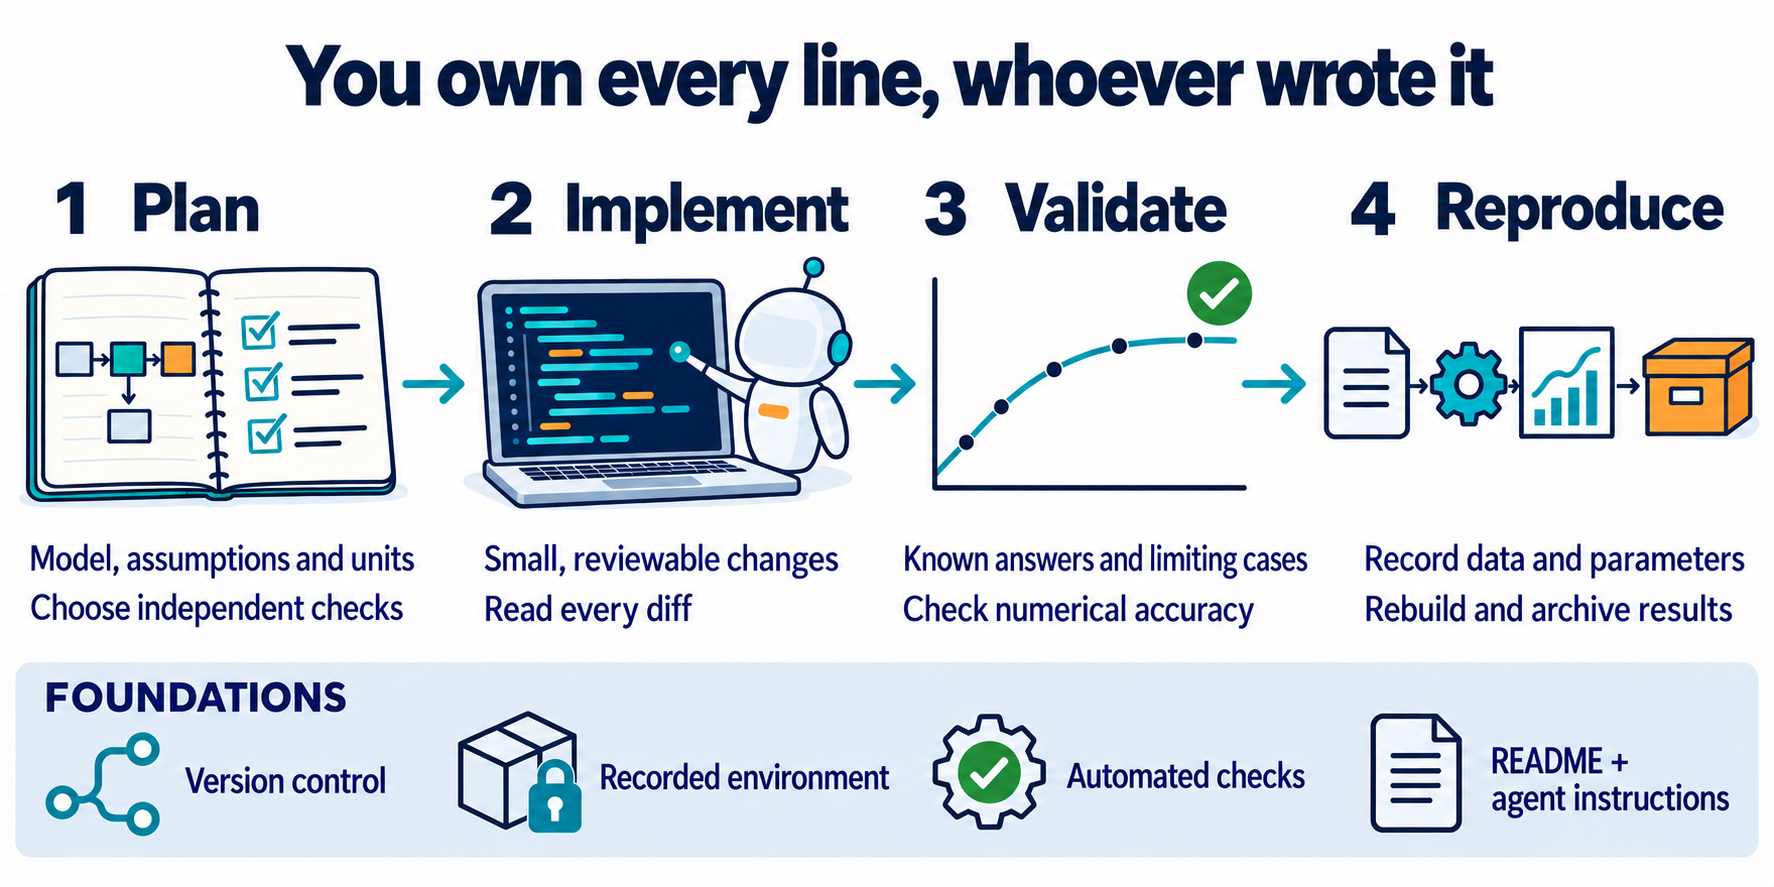
\includegraphics[height=0.95\textheight,width=\textwidth,keepaspectratio]{summary.png}}
  \note[item]{Choose how you will check a result before delegating
    it. Scientific checks
    include analytic answers, limiting cases and
    simulate-and-recover, independently of the
  implementation.}
  \note[item]{Version control, a recorded environment, automated
    checks and clear instructions
    support the whole workflow. You remain responsible for the science
  and the code.}
\end{frame}

\end{document}
